% a gem of a website: https://mpetroff.net/files/beamer-theme-matrix/
\documentclass[xcolor={dvipsnames,svgnames}]{beamer}
\usetheme{PaloAlto}
\usecolortheme{spruce}
\usepackage[utf8]{inputenc}
\usepackage{enumerate}
\usepackage{amsmath}
\usepackage{amsthm}
\usepackage{amssymb}
\usepackage{amsbsy}
\usepackage{amsfonts}
\usepackage{hyperref}
\usepackage{tikz}
\usepackage{verbatim}
\usepackage{mathtools}
\usepackage{macros}
\usepackage{float}
\usepackage{caption}
\usepackage{subcaption}
\usepackage{xcolor,graphicx}
\usepackage{animate}
\usepackage{tikz}
\usetikzlibrary{positioning}
\setbeamertemplate{caption}[numbered]
\DeclareUnicodeCharacter{2212}{-}
\usepackage{tikz-cd}
\usepackage{flowchart}
\usetikzlibrary{
  shapes,
  arrows.meta, % supersedes arrows
  calc,automata,positioning,fit,quotes}
  \tikzset{
  line/.style={draw, -Latex}
}
\tikzstyle{arrow} = [thick,->,>=stealth]
\captionsetup{font=scriptsize,labelfont={bf,sf}}
\captionsetup[subfigure]{font=scriptsize,labelfont=scriptsize}

\makeatletter
  \setbeamertemplate{sidebar \beamer@sidebarside}%{sidebar theme}
  {
    \beamer@tempdim=\beamer@sidebarwidth%
    \advance\beamer@tempdim by -6pt%
    \insertverticalnavigation{\beamer@sidebarwidth}%
    \vfill
    \ifx\beamer@sidebarside\beamer@lefttext%
    \else%
      \usebeamercolor{normal text}%
      \llap{\usebeamertemplate***{navigation symbols}\hskip0.1cm}%
      \vskip2pt%
    \fi%
}%
\title{Manifold Structure of High-Dimensional Data in Artificial and Biological Neural Networks}
\author{Zhang Liu\\ Supervisor: Prof.~Francesca Spagnuolo\\Cosupervisors: Prof.~Steven W.~Zucker, Dr.~Luciano Dyballa\\ Yale Zucker Lab}

\date{\today}
\logo{\includegraphics[width=.075\textwidth]{YaleNUS_workmark_solid.eps}}
\begin{document}

\begin{frame}
\titlepage
\end{frame}

\section{Our Goals}
\begin{frame}{Our goals (neurobiological): \\modeling the visual system}
\begin{itemize}
    \item Primary visual cortex (V1)
    \begin{figure}[H]
            \centering
                \includegraphics[width=0.25
                \textwidth]{figures-models/v1.jpg}
                \caption{Visual input goes from the eye to primary visual cortex (V1).\\ (Adapted from Polyak (1957))}
            \end{figure}     
        \item How is the structure of neurobiological networks in V1 similar/different from artificial neural networks (ANNs)?
        \item  In the end, the goal is to come up with more accurate models of the visual system.
\end{itemize}
\end{frame}
\begin{frame}{Our goals (computational/mathematical): \\learning the neural manifolds}
\begin{itemize}
        \item \textit{Neural manifolds}: (informal) clusters of neurons grouped by their firing patterns in response to a given visual stimulus. 
        \item Compare the neural manifolds for biological neural networks vs artificial neural networks: 
        
        Convolutional Neural Networks (CNNs), Recurrent Neural Networks (RNNs) and the recent Transformer and Perceiver networks.
\end{itemize}
\end{frame}

\begin{frame}{Significance}
\begin{itemize}
    % \item Artificial neural networks have proved capable of many vision tasks at a level competitive to biological systems. 
    \item Misconception: ``CNNs works like the visual cortex."
    \item Whether artificial and biological neural networks use the same computational strategies \textbf{remains an open question.} \cite{Gwilliams221630}
    \item Modeling the visual system is an important task:
    \begin{itemize}
        \item for \textbf{neuroscience}: scientific understanding of the brain
        \item for \textbf{AI}: reverse-engineering, e.g., 
        
        LeCun, Bengio, \& Hinton: ``CNNs have their roots in the neocognitron" which was one of the earliest computational models of the visual system. \cite{lecun_deep_2015}
    \end{itemize}
\end{itemize}
\end{frame}

\section{The Method}
\begin{frame}{Summary of the method}
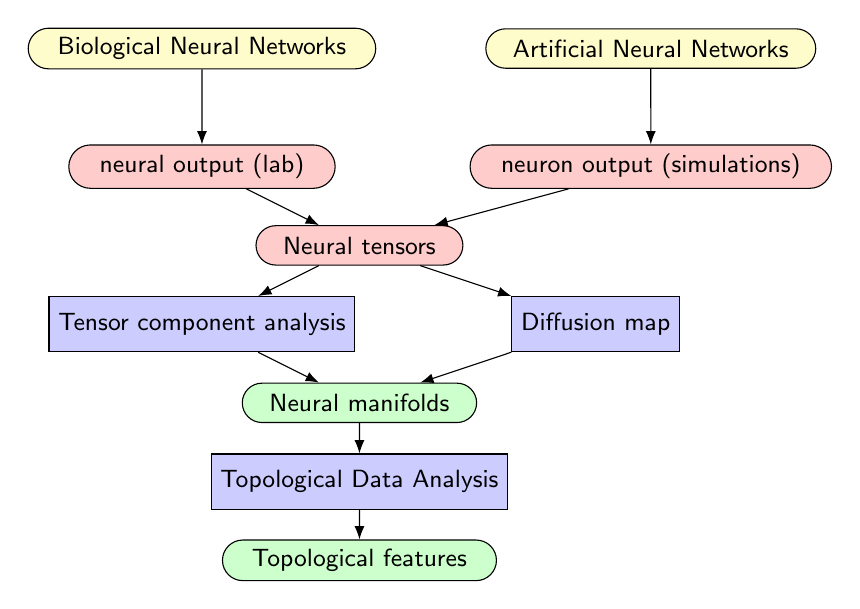
\begin{tikzpicture}[font={\sf \small}]
 \def\smbwd{2cm}
  \node (BNN) at (-3,0.5) [draw, terminal, minimum width=\smbwd,  fill=yellow!20, minimum height=0.5cm] {Biological Neural Networks}; 
  \node (ANN) at (2.7,0.5) [draw, terminal, minimum width=\smbwd,  fill=yellow!20, minimum height=0.5cm] {Artificial Neural Networks}; 
  %------------
  \node (experimental) at (-3,-1) [draw, terminal, minimum width=\smbwd,  fill=red!20, minimum height=0.5cm]{neural output (lab)};
  \node (artificial) at (2.7,-1)[draw, terminal,minimum width=\smbwd,  fill=red!20, minimum height=0.5cm]{neuron output (simulations)};
  %------------
  \node (tensors) at (-1,-2) [draw, terminal, minimum width=\smbwd,  fill=red!20, minimum height=0.5cm] {Neural tensors}; 
  %------------
  
  \node (TCA) at (-3,-3) [draw, process, minimum width=\smbwd, fill=blue!20, minimum height=0.7cm] {Tensor component analysis};
  \node (diffusion) at (2,-3) [draw, process, minimum width=\smbwd, fill=blue!20, minimum height=0.7cm] {Diffusion map};
  %------------
  
  \node (manifolds) at (-1,-4) [draw, terminal, minimum width=\smbwd,  fill=green!20, minimum height=0.5cm] {Neural manifolds};
  
  \node (TDA) at (-1,-5) [draw, process, minimum width=\smbwd, fill=blue!20, minimum height=0.7cm] {Topological Data Analysis};
   
 \node (topology) at (-1,-6) [draw, terminal, minimum width=\smbwd,  fill=green!20, minimum height=0.5cm] {Topological features};
 
  %------------
  
  
 \path [line](BNN) -- (experimental);
 \path [line](ANN) -- (artificial);
 \path [line](tensors) -- (TCA);
 \path [line](tensors) -- (diffusion);
 \path [line](experimental) -- (tensors) ;
 \path [line] (artificial) -- (tensors) ;
 \path [line](diffusion) -- (manifolds);
 \path [line](TCA) -- (manifolds);
  \path [line](manifolds) -- (TDA);
  \path [line](TDA) -- (topology);
 \end{tikzpicture}
 
\end{frame}

% \begin{frame}{The bigger picture: Modeling V1}
%     \begin{itemize}
%         \item convolution operator: at simple cells. The convolution of $K(t)$ (e.g. a kernel) and $g(t)$ (e.g. an image), $K \ast g$ is defined by 
%         \begin{align}
%             [K \ast g](t) = \int^t_0 K(u)g(t-u)du.
%         \end{align}
%         \item pooling operator (taking the average or maximum): at complex cells 
%     \end{itemize}  
% \end{frame}


% \begin{frame}{The problem: modeling visual perception}
% \begin{itemize}
%     \item Hierarchy model by Hubel and Wiesel (1965)
%      \begin{figure}[H]
%         \centering
%             \includegraphics[width=0.8\textwidth]{figures-models/hierarchy-model.jpg}
%             \caption{Hierarchical model of V1. (Adapted from Prof. Zucker's notes)}
%         \end{figure} 
% \end{itemize}
% \end{frame}

\begin{frame}{Data: from lab experiments}
    \begin{itemize}
        \item Visual stimuli of artificial gratings are flashed in front of the mouse.
        \item Each visual stimuli are shifting in 8 directions over time.
        \item Neuron output is recorded with electrodes and encoded in peristimulus (PSTH) diagrams.
        \item Each PSTH diagram shows the firing rate of one neuron over time for 8 directions. Brighter pixels indicate higher firing rates.
    \end{itemize} 

   \begin{figure}
        \centering
            \includegraphics[width=0.55\textwidth]{presentation/Slide5.jpg}
            \caption{Visualising neural data from lab experiments.}
    \end{figure}
\end{frame}
\begin{frame}{Data: from computational simulations}
    \begin{itemize}
        \item Input natural images of different objects (e.g. cars, cats, and dogs) to Artificial Neural Networks (ANNs).
        \item Compute output (numerical values) from neuron units.
    \end{itemize}
    % add image
    \begin{figure}
        \centering
            \includegraphics[width=0.9\textwidth]{Slide1.jpg}
            \caption{Computing output of one neuron unit in the ANNs given 10 input cat images.}
    \end{figure}
    % add output
\end{frame}


% \begin{frame}{Challenges in neural data analysis in V1}
%     \begin{itemize}
%         \item Limited experimental results\dots
        
%         \item[] Solution: use Artificial Neural Networks (ANNs) to generate artificial neural tensors.
        
%         \item High-dimensional\dots
        
%       \item[] Solution: use dimensionality reduction methods like tensor component analysis and diffusion map. 
        
%         \item Complex geometric structure\dots 
        
%         \item[] Solution: use analytic tools from differential geometry.
%     \end{itemize}
% \end{frame}

% \begin{frame}{Principal Component Analysis (PCA)}

% \begin{itemize}
%     \item PCA is a common linear dimensionality reduction method.
%     \item PCA finds the principal components, i.e., the eigenvectors that correspond to the largest variance.
%     \item The first principal component contain most of the information about the original data. We will not lose too much if we approximate our data by taking just the first few principal components.
% \end{itemize}
% % (With Acrobat reader, an animation of the plots generated during the training process can be viewed below)
% \begin{figure}[H]
% \begin{minipage}[b]{0.8\textwidth}
% \animategraphics[width=\textwidth,loop,autoplay]{8}{pca-animation/frame_}{000}{129}
% \caption{Animation adapted from \cite{pca-se}.}
% \end{minipage}
% \end{figure}  
% \end{frame}

\begin{frame}{Tensors}
\begin{defn}[Tensors]
    An $N$-way tensor is an element of the tensor product of $N$ vector spaces. 
    \begin{itemize}
        \item $1$-way tensor = vector, $v = [v_1 \quad v_2 \quad \dots \quad v_n]^T.$
        \vfill
        \item $2$-way tensor = matrix, 
        $A = \left(\begin{matrix}
        A_{1 1} & A_{1 2} & \dots & A_{1 n}\\
        \vdots & \vdots & \vdots & \vdots \\ 
        A_{m 1} & A_{m 2} & \dots & A_{m n}
        \end{matrix}
        \right).$
        \vfill
        \item $3$-way tensor of dimension $I$-by-$J$-by-$K$:
    \begin{figure}[H]
    \centering
    \includegraphics[width=0.35\textwidth]{figures-tensor/tensor-vis.png}
    \end{figure} 
    \end{itemize}
    \end{defn}
\end{frame}

\begin{frame}{Neural tensors}
\begin{defn}[Neural population response]
    Suppose $\mathcal{S}$ is a set of $S$ visual stimuli (e.g., images) $\mathcal{S} = \{s_1, s_2,\dots, s_S\}$, each having $T$ number of transformations (translations or rotations). The \underline{neural population response} of a set of $N$ neurons to a stimulus $m_i$ over all transformations is $\mathcal{N} = \{\vec{n}_1, \vec{n}_2, \dots, \vec{n}_N\},$ where $\vec{n}_i \in \mathbb{R}^T$. 
\end{defn}
\begin{defn}[Neural tensors]
    Each \underline{neural tensor} encodes the neural population response of a set of neurons to a set of stimulus over all transformations. It is thus a $3$-way tensor of dimension $N$-by-$S$-by-$T$.
    
    % The neural spiking data set used in this project is represented by a $3$-way tensor of dimension $698$-by-$6$-by-$264$. The three dimensions represent the following respectively: there are in total $698$ neurons $6$, $6$ types of visual stimuli, and $264$ number of pixels in the PSTH diagram.
\end{defn} 
\end{frame}
\begin{frame}{Neural manifolds}
    \begin{defn}[Manifold]
    A \underline{manifold} is a topological space that ``locally" resembles Euclidean space. 
    \end{defn}
    \begin{minipage}[t]{.45\linewidth}  
    \begin{figure}
     \includegraphics[width=\textwidth]{presentation/manifold.jpg}
    \end{figure} 
    \end{minipage}
    \hfill
      \begin{minipage}[t]{.45\linewidth}   
      \begin{figure}
      \includegraphics[width=\textwidth]{figures/embeddings/embedding-lab.png}
            \end{figure} 
    \end{minipage}
\begin{defn}[Neural manifolds]
Clusters of neurons grouped by their firing patterns in response to a given visual stimulus. The distance defined on the neural manifolds indicate how similarly the neurons respond.
\end{defn}
\end{frame}

\begin{frame}{Dimensionaliy Reduction}
% the manifold hypothesis:
\begin{asm}[The Manifold Hypothesis]
Real-world high-dimensional data lie on low-dimensional manifolds embedded within the high-dimensional space. \cite{deepai_2019}
\end{asm}
% main idea behind manifold learning:
\begin{itemize}
    \item \textbf{Image data} are high-dimensional (the number of pixels), but can be reparameterized with much smaller number of variables (feature extraction).
    \item \textbf{Neural data} are high-dimensional, but the neural connections constrain the possible neural firing patterns to a low-dimensional manifold spanned by a few independent patterns. \cite{gallego_neural_2017}
\end{itemize}
\end{frame}


\begin{frame}{Linear dimensionality reduction: tensor component analysis + k-means clustering}
    \begin{figure}[H]
        \centering
            \includegraphics[width=0.8\textwidth]{figures-tensor/cp-decomp.png}
            \caption{Intuition for tensor component analysis. (Adapted from \cite{Kol2009}.)}
        \end{figure} 
    \begin{figure}[H]
        \centering
            \includegraphics[width=0.6\textwidth]{presentation/figures-tensor/kmeans.png}
            \caption{Intuition for k-means clustering.}
        \end{figure} 
\end{frame}

\section{The Results}
\begin{frame}{Demo: apply tensor component analysis to face image data (from 1000 face images to 5 features)}
    \begin{figure}[H]
        \centering
            \includegraphics[width=0.9\textwidth]{Slide2.jpg}
            \caption{First 5 tensor factors for face image data.}
        \end{figure}
    \begin{figure}[H]
        \centering
            \includegraphics[width=0.5\textwidth]{figures/embeddings/embedding-face.png}
            \caption{Face embedding.}
        \end{figure} 
\end{frame}

\begin{frame}{Demo: apply tensor component analysis to face image data (face images by cluster)}
      \begin{figure}[H]
            \centering
            \begin{subfigure}[b]{0.45\textwidth}
                \includegraphics[width=\textwidth]{figures-face-results/face14.png}
            \end{subfigure}
            \hfill 
            \begin{subfigure}[b]{0.45\textwidth}
                \includegraphics[width=\textwidth]{figures-face-results/face15.png}
            \end{subfigure}
            \hfill
            \begin{subfigure}[b]{0.45\textwidth}
                \includegraphics[width=\textwidth]{figures-face-results/face16.png}
            \end{subfigure}
            \hfill
            \begin{subfigure}[b]{0.45\textwidth}
                \includegraphics[width=\textwidth]{figures-face-results/face17.png}
            \end{subfigure}
            \caption{Some arbitrary clusters showing the results of TCA for face data.}
            \end{figure} 
\end{frame}

%% NEED TO CHANGE AND EXPLAIN!!! 
\begin{frame}{Results: first five principal components from biological neural tensor}
    \begin{figure}[H]
        \centering
            \includegraphics[width=\textwidth]{Slide3.jpg}
            \caption{First 5 tensor factors for neural data.}
        \end{figure} 
\end{frame}
\begin{frame}{Results: visualize neural manifolds from biological neural tensor}
    \begin{figure}[H]
        \centering
            \includegraphics[width=\textwidth]{figures/embeddings/embedding-lab.png}
            \caption{Neural manifolds: clusters of neurons grouped by firing patterns, each point represent a neuron.}
        \end{figure} 
\end{frame}
\begin{frame}{Results: look inside the neural manifolds}
      \begin{figure}[H]
            \centering
            \begin{subfigure}[b]{\textwidth}
                \includegraphics[width=0.95\textwidth]{figures-retina-results/cluster20.png}
                \caption{PSTH diagrams showing responses of neurons within some arbitrary cluster to stimuli of type 1.}
            \end{subfigure}
            \vfill 
            \begin{subfigure}[b]{\textwidth}
                \includegraphics[width=0.95\textwidth]{figures-retina-results/cluster10.png}
                \caption{PSTH diagrams showing responses of neurons within a different cluster to stimuli of type 1.}
            \end{subfigure}
            \end{figure} 
\end{frame}

\begin{frame}{Results: first five principal components from artificial neural tensor}
      \begin{figure}[H]
        \centering
            \includegraphics[width=\textwidth]{artificial-tensor/results/nonneg_factors_3D.png}
            \caption{First 5 tensor factors for artificial neural data.}
        \end{figure} 
\end{frame}

\begin{frame}{Results: visualize neural manifolds from artificial neural tensor}
    \begin{figure}[H]
        \centering
            \includegraphics[width=\textwidth]{artificial-tensor/results/TCA_3D.png}
            \caption{Neural manifolds.}
        \end{figure} 
\end{frame}

\begin{frame}{Non-linear dimensionality reduction: diffusion map}
        \heading{Applying diffusion map to synthetic spiral data and MNIST handwritten digits images data:}

    \begin{minipage}[t]{.45\linewidth}  
    \begin{figure}
            \includegraphics[width=0.6\textwidth]{spiral.png}
            \caption{Visualising the original spiral data.}
        \end{figure} 
      \begin{figure}         \includegraphics[width=0.6\textwidth]{spiral-unroll.png}
            \caption{First non-trivial coordinate function.}
            \end{figure} 
    \end{minipage}
    \hfill
      \begin{minipage}[t]{.45\linewidth}   
    \begin{figure}
            \includegraphics[width=0.4\textwidth]{mnist-vis.png}
            \caption{Sample data from the MNIST.}
        \end{figure} 
      \begin{figure}
                \includegraphics[width=0.6\textwidth]{mnist.png}
            \caption{First two non-trivial coordinate functions.}    
            \end{figure} 
    \end{minipage}
\end{frame}

\begin{frame}{Putting it all together and next steps:}
\begin{figure}[H]
        \centering
            \includegraphics[width=1.2\textwidth]{Slide4.jpg}
        \end{figure} 
\end{frame}

% \begin{frame}{More on convolution and kernels} 

% We can define the kernel and convolve it with an image so as to modify the image in a desired way. For example: 
% \begin{itemize}
%     \item The Gaussian kernel blurs the image:
%     \begin{figure}[H]
%         \centering
%             \includegraphics[width=0.8\textwidth]{figures-face-results/face_gaussian.png}
%         \end{figure} 
%     \item The Laplacian of Gaussian kernel sharpens the image:
%     \begin{figure}[H]
%         \centering
%             \includegraphics[width=0.8\textwidth]{figures-face-results/face_laplacian_overlay.png}
%         \end{figure} 
% \end{itemize}
%     % Note that the ``sharpening" here is not the inverse of ``blurring." We would need a ``deblurring" kernel. 
% \end{frame}

% \begin{frame}{Bonus Slide: Recent Progress}
% For 

% \end{frame}
% \begin{frame}{Alternative to the hierarchy model: recurrent models}
% \textbf{Recurrent models: study networks of cortical connections instead of individual cells. }

% Recurrent computation: 
% \begin{align}
%     S_i(\lambda) = \sum_{j \in \text{neigh}(i)}\sum_{\lambda^\prime \in \Lambda(j)} r_{i,j}(\lambda, \lambda^\prime) p_j(\lambda^\prime)\\
%     P^{t+1}_i(\lambda) = \prod_k [P_i^t(\lambda) + \delta s_i(\lambda)]
% \end{align}

%     \begin{figure}[H]
%     \begin{subfigure}{0.45\textwidth}
%       \centering
%       \subfloat[]{\includegraphics[width=2in]{figures-models/cortical2.png}}
%     \end{subfigure}
%     \hfill
%     \begin{subfigure}{0.45\textwidth}
%       \centering
%       \subfloat[]{\includegraphics[width=2in]{figures-models/cortical1.png}}
%     \end{subfigure}
%     \end{figure}
% \end{frame}

% \begin{frame}{Bonus slide: modeling lateral inhibition}
% Algebraic model for lateral inhibition: 
% \begin{align}
%     F_i = e_i - \sum_{j \in \text{neighbors}(i)}\alpha_{i,j} \quad e_j, \quad \alpha_{i,j} \in \mathbb{R}^{+}.
% \end{align}
%     \begin{figure}[H]
%         \centering
%             \includegraphics[width=0.7\textwidth]{figures-models/lateral-inhibition.png}
%         \end{figure} 
% \end{frame}


\begin{frame}{Bonus Slide:)}
\begin{exampleblock}{}
  {\large \textit{Look for the bare necessities\\
            The simple bare necessities\\
            Forget about your worries and your strife\\
            I mean the bare necessities\\
            Old Mother Nature’s recipes\\
            That bring the bare necessities of life}}
  \vskip2mm
  \hspace*\fill{\small--- Baloo’s song [The Jungle Book]}
\end{exampleblock}
  \begin{figure}
  \href{https://www.youtube.com/watch?v=9ogQ0uge06o}{ \includegraphics[width=0.45\textwidth]{presentation/bare-necessities.jpg}}
            \end{figure} 
\end{frame}

\begin{frame}{Acknowledgements}
I would like to thank my supervisor Prof.~Francesca Spagnuolo  and co-supervisor and mentor Prof.~Steven W. Zucker and Dr.~Luciano Dyballa for their generous guidance and advice. They have made possible the many serendipitous moments in this project. 
\end{frame}
\begin{frame}{Artificial neural tensors}
        \begin{figure}
            \includegraphics[width=\textwidth]{figures/artificial/vgg16.png}
            \caption{VGG-16}
        \end{figure} 
\end{frame}
\section{References}
\begin{frame}{References}
\bibliographystyle{plain}
\bibliography{biblio}
\end{frame}

\end{document}